\RequirePackage[l2tabu, orthodox]{nag}
\documentclass[a4paper, twocolumn]{article}
\usepackage[utf8]{inputenc}
\usepackage[T1]{fontenc}
\usepackage[pdftex, hidelinks,
            pdftitle={Behaviour Tree Evolution by Genetic Programming},
            pdfauthor={Martin Estgren and Erik S. V. Jansson},
            pdfsubject={Artificial Intelligence - Genetic Programming},
            pdfkeywords={artificial intelligence, genetic programming,
                         behaviour trees, a-star, shooter}]{hyperref}

\usepackage{bm}
\usepackage{caption}
\usepackage{listings}
\usepackage{booktabs}
\usepackage{mathtools}
\usepackage{algorithmic}
\usepackage{graphicx}
\usepackage{courier}
\usepackage{amsmath}
\usepackage{amssymb}
\usepackage{algorithm}
\usepackage[capitalize, noabbrev]{cleveref}
\usepackage[activate={true, nocompatibility}, final,
            tracking=true, kerning=true, spacing=true,
            factor=1100, stretch=10, shrink=10]{microtype}

\newcommand\blfootnote[1]{%
    \begingroup
        \renewcommand\thefootnote{}\footnote{#1}%
        \addtocounter{footnote}{-1}%
    \endgroup
}

\DeclareCaptionFormat{modifiedlst}{\rule{\textwidth}{0.85pt}\\[-2.9pt]#1#2#3}
\captionsetup[lstlisting]{format =  modifiedlst,
labelfont=bf,singlelinecheck=off,labelsep=space}
\lstset{basicstyle=\footnotesize\ttfamily,
        breakatwhitespace = false,
        breaklines = true,
        keepspaces = true,
        language = Java,
        showspaces = false,
        showstringspaces = false,
        frame = tb,
        numbers = left,
        numbersep = 5pt,
        xleftmargin = 16pt,
        framexleftmargin = 16pt,
        belowskip = \bigskipamount,
        aboveskip = \bigskipamount,
        escapeinside={<@}{@>}}

\title{\textbf{Behaviour Tree Evolution by Genetic Programming}\\
       \Large{\emph{-- Learning Novel Bot Behaviours in a 2D Top-Down Arena Shooter --}}}
\author{{\textbf{Martin Estgren}} \;\;\;\;\;\;\;\;\;\, {\href{mailto:mares480@student.liu.se}
                                                       {\texttt{<mares480@student.liu.se>}}} \\
        {\textbf{Erik S. V. Jansson}} \;\;\;\;         {\href{mailto:erija578@student.liu.se}
                                                       {\texttt{<erija578@student.liu.se>}}} \\~\\
        {Linköping University, Sweden}\vspace{-2.0ex}}

\begin{document}
    \maketitle
    \section*{Abstract}

    Behaviour trees are a popular model for representing the decision-making and plan execution process for NPCs in video games. These are built by hand, and require expertise to craft. They don't adapt well to other environments, and often require a custom BT.

    In this paper we demonstrate how to generate the BTs by using genetic programming; allowing us to essentially evolve novel behaviours automatically in our testbed. Instead of specifying low-level actions and conditions, we use high-level definitions. This leads to faster fitness convergence, and also allows us to skip the bloat control and tree pruning steps used by other methods. Results show that the evolved BT beats our hand-crafted BT by the \(5^{th}\) generation. \footnotemark[1]

    \vspace{1.0em}

    \begingroup
    \def\addvspace#1{}
    \tableofcontents
    \endgroup
    \newpage

    \newpage % Next column...
    \nocite{*} % Include all.
    \bibliographystyle{abbrv}
    \bibliography{report}
    \footnotetext[1]{Repository: \url{https://github.com/sci10n/Quake2D}}
    \thispagestyle{empty}
    \clearpage
    \addtocounter{page}{-1}

    \section{Introduction} \label{sec:introduction}

    In interactive media such as video games, there is often a need for simulating seemingly complex agent behaviours in soft real-time. In a modern fast-paced computer game for example, the render, physics and artificial intelligence updates all need to complete in a total of less than 16ms to provide a half-decent experience. These requirements have spawned some clever techniques to enable complex behaviours for autonomous agents while minimizing computation.

    These techniques often require manual behaviour definition, and in some cases, are hard to extend when new behaviours are needed for a game, as shown by industry researchers, e.g. \emph{Dawe et al}~\cite{dawe2014overview}, regarding the finite state machine architecture. In this project we have explored how one of the more widely used techniques, \emph{behaviour trees}, can be extended to allow for not only hand-crafted complex behaviors, but for organic behaviours tailored to the specific game domain by using \emph{reinforcement learning}. More specifically, we evolve behaviour trees with \emph{genetic programming}, which spawn behaviour tree offspring.

    Alongside the proposed method in \cref{sec:proposed_approach}, a testbed consisting of a top-down arena shooter was built. It features a sufficiently complex environment to support interesting behaviours by the enemy bot. We describe the features of our testbed in \cref{sec:implementation_details}.

    This report starts off in \cref{sec:background_theory} by giving a brief overview of the relevant techniques and related work necessary to follow our reasoning and findings. In \cref{sec:implementation_details} we describe the details needed to implement these techniques in practice, along with the testbed architecture we've used. This gives the reader information on any peculiarities and pit-falls. We follow this by showing in \cref{sec:results_and_screenshots} the testbed, and give some generated offspring generated by our method along with measurements of its efficiency. Finally, we reflect on our method, giving downsides, and present some possible future work in \cref{sec:discussion_and_outlook}.

    \vspace{-0.8em}

    \subsection{Proposed Approach} \label{sec:proposed_approach}

    Apply \emph{genetic programming} to the \emph{behaviours trees} by creating \emph{high-level actions and conditions} nodes. Ideally this should allow for faster convergence rates and somewhat shallower generated behaviour trees, eliminating the need for bloat control and pruning. Since BTs are trees, the \emph{mutation mechanism} should modify \emph{control-flow structure} and \emph{leaf-node settings}, while the \emph{crossover mechanism} will swap sub-trees.

    \section{Background Theory} \label{sec:background_theory}

    For an autonomous agent to give the illusion of intelligence, many different systems and techniques need to interact with each other. In this chapter we describe the theory behind our three primary systems: \emph{behaviour trees}, \emph{path finding} \& \emph{genetic programming}.

        \subsection{Behaviour Trees} \label{sec:behaviour_trees}

        Defining an accurate \emph{automatic planner} model is often impractical and usually overkill for real-world applications. Especially in games, where very simple models are enough to give the illusion of intelligence. In games, the most well-known \emph{behaviour selection algorithms} are \emph{FSMs}, \emph{GOAPs}, \emph{HTNs} and \emph{BTs} \cite{dawe2014overview}.

        \emph{Finite State Machines (FSMs)} are simple but are hard to extend with additional states, making the amount of transitions to increase exponentially \cite{dawe2014overview}. While both \emph{GOAP (Goal-Oriented Action Planner)} and \emph{HTN (Hierarchical Task Network)} are powerful models, these don't allow agents to explore new task definitions, and ``only'' provide an agent with novel ways of solving an already defined set of task defs.

        \emph{Behaviour Trees (BTs)} on the other hand, when comparing to FSMs, provide advantages in terms of modularity, reactiveness and scalability. And more importantly, since they are a type of tree, allow for integration with the genetic programming approach. They were first popularized by the game \emph{Halo 2}, but are now used in other area as well, such as robotics.

        In the \emph{Behaviour Tree Starter Kit}~\cite{champandard2014behaviour} and also in \emph{Chris Simpson's Gamasutra article}~\cite{simpson2014behavior}, the BT is a tree-like data structure which describes the decision-making process of the agent. It's evaluated pre-order from the root of the tree in each logic update tick.

        \begin{figure}[H]
            \centering
            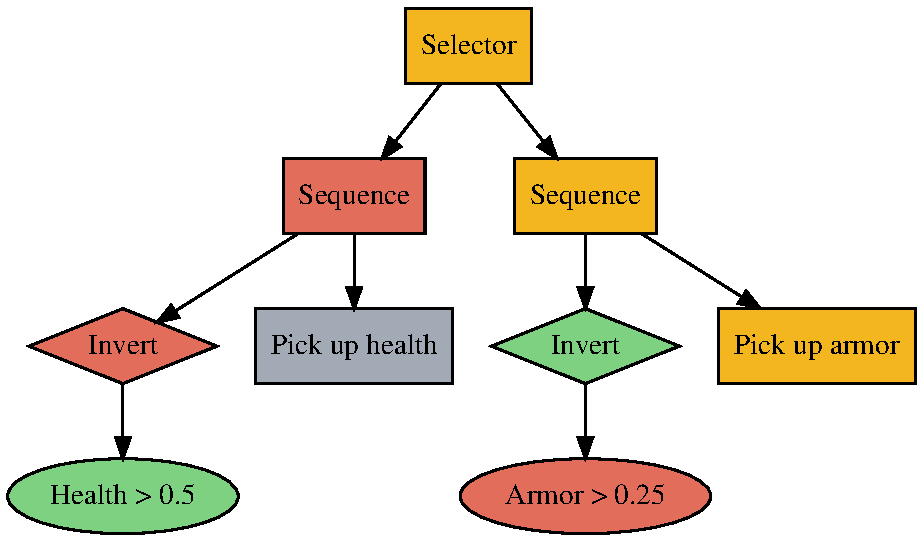
\includegraphics[width=\linewidth]{share/behaviour_tree.pdf}
            \caption{Example of Hand-Crafted Behaviour Tree}
            \label{fig:behaviour_tree}
        \end{figure}

        Below you'll find the most common concrete types of nodes in a behaviour tree, as those in \emph{BTSK}~\cite{champandard2014behaviour}. Only \emph{action} and \emph{condition nodes} are \emph{leaf-nodes}, all others are either \emph{composite or decorator nodes} that have one or more children (hence, never a leaf node).

        \begin{itemize}
            \item{\textbf{Selector:} executes children from left \(\rightarrow\) right until \emph{one child} is found to be either \emph{running} or has already \emph{succeeded}, and returns this status. Otherwise, if none matches, it returns a \emph{failure}.}
            \item{\textbf{Sequence:} executes children from left \(\rightarrow\) right until \emph{one child} is found to be either \emph{running} or \emph{failed}, and returns this status. If \emph{all children} have \emph{succeeded}, then also set status to \emph{success}.}
            \item{\textbf{Inverter:} executes the child node and \emph{inverts the resulting state} when it has finished running.}
            \item{\textbf{Succeeder:} when child has finished running, returns \emph{success} regardless of the child's status.}
            \item{\textbf{Condition:} a leaf-node that queries the world state, if the query returns true, we give \emph{success}, if it's false, we instead give \emph{failure}. This node is usually instantaneous, and can't be \emph{running}.}
            \item{\textbf{Action:} a leaf-node which modifies the world state, and returns \emph{success} if the action had the intended side-effect, \emph{failure} if couldn't complete or failed the action and \emph{running} if not done yet.}

        \end{itemize}

        We find that it's easier to understand behaviour trees with an example. We'll be using the tree in \cref{fig:behaviour_tree} as an example (it was produced within our testbed using a Graphviz library for Java). The yellow nodes means the node state is \emph{running}, the \emph{red} nodes have \emph{failed}, and \emph{green} nodes have \emph{succeeded}.

        At a high-level, this BT checks the agent's health and armor, and if it's below a threshold, it will go and pick up the crates which replenish these stats.

        It does this by starting at the root node, \emph{selector}, and executing the left child, the \emph{sequence}. It will also execute its left child, which is the \emph{inverter}. At last we reach a leaf-node, the \emph{health condition node}. This will probe the world for the state of the agent, and return \emph{success} because we've found that it's above 50\%. This result will propagate upward to its parent, the inverter, which will set its state to \emph{failed} (inverting the result of the child). We're back at the left sequence, and because one of the children have failed (the inverter), the sequence has \emph{failed} as well, and won't run the right child. Execute right node...

        \subsection{Path Finding with A*} \label{sec:path_finding}

	Agent path finding is done using the \emph{A*} graph traversal algorithm proposed by Peter E. Hart, Nils J. Nilsson, and Bertram Raphael ~\cite{hart1968formal} as an extension to \emph{Dijkstra's algorithm} which, given an \emph{admissible heuristic} and non-negative costs, will find the path from a node \(n_0\) to a node \(n_g\), with the lowest cost.
	
    Calculating the expected cost of a path, like this: \(n_0 \rightarrow n_k \rightarrow n_g\), from \(n_0\) to \(n_g\) via \(n_k\) can be done with the following traversal function:
	\begin{equation*}
		f(n_k) = g(n_k) + h(n_k)
	\end{equation*}	
	where \(g(n_k)\) is the true cost from \(n_0\) to node \(n_k\) and \(h(n_k)\) is a heuristic approximation of the cost from \(n_k\) to \(n_g\). This allows us to explore the potentially most optimal paths before expanding the other ones.

        In this project, the \emph{Euclidean distance} is used as the heuristic \(h(n_k)\). This since the path finding is performed in a search-space where each node is defined as a point in the testbed's 2-D world-space.

    Additionally, compared to regular \emph{A*}, the path-finder also utilizes an \emph{influence map} to help the agent avoid ``suicidal paths'', even if the selected path is optimal given the heuristic function. Our \emph{influence map}, like the ones shown in \emph{Dave Mark}~\cite{mark2015modular}, take into account the visibility of each node in relation to the adversarial game agents' line-of-sight, and therefore updates the expected cost as:
	\begin{equation*}
		f(n_k) = g(n_k) + h(n_k) + i(n_k)
	\end{equation*} 
    where \(i(n_k)\) is the cost introduced by the influence map. This gives the the result that nodes within the adversarial agent's line-of-sight have a much higher associated traversal cost, and should be avoided. 
    \begin{minipage}{\linewidth}        	
    \centering
	\begin{minipage}{0.45\linewidth}
	\begin{figure}[H]
        \centering
		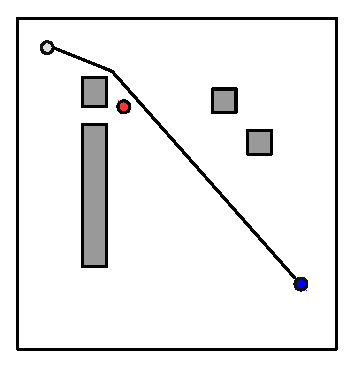
\includegraphics[width=\linewidth]{share/bad.eps}
		\caption{optimal path}
		\label{fig:optimal_path}
        \end{figure}
	\end{minipage}
	\hspace{0.00\linewidth}
	\begin{minipage}{0.45\linewidth}
	\begin{figure}[H]
        \centering
		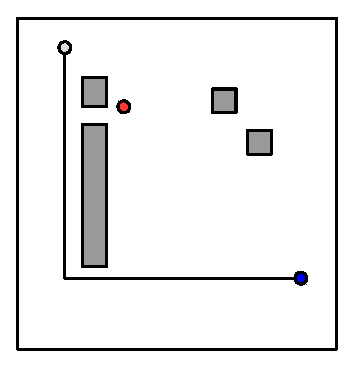
\includegraphics[width=\linewidth]{share/good.eps}
		\caption{tactical path}
		\label{fig:smart_path}
	\end{figure}
	\end{minipage}
\end{minipage}

\vspace{0.5em}

    Above are two example figures: \cref{fig:optimal_path} shows an optimal path using regular \emph{A*}, and the other, \cref{fig:smart_path} shows the optimal path when taking into account the influence map; sneaking behind cover.
	
	\subsection{Genetic Programming} \label{sec:genetic_programming}

    In many scenarios you try to optimize the input of a function: \(f(x_0,x_1,...,x_n)\), where some or all of the inputs are of a discrete nature (ordinal or nominal values). These types of problems are often hard to optimize using techniques developed for continuous variables, such as \emph{gradient ascent/descent}.

	\emph{Genetic programming} is a technique that was introduced by \emph{Barricelli et al}~\cite{barricelli1954esempi}, as a way to optimize computer programs by encoding the parameters to be optimized as \emph{genetic representations} which could be processed by traditional \emph{evolutionary algorithms}.

	\begin{figure}[H]
        \centering
		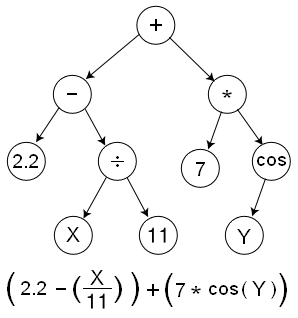
\includegraphics[width=0.5\linewidth]{share/Genetic_Program_Tree.png}
		\caption{The \emph{genetic representation} is often done using a tree-like structure in \emph{genetic programming}.}
		\label{fig:genetic_representation}
	\end{figure}

	The most general form of \emph{evolutionary algorithms} can be described in the following few steps:
    \begin{enumerate}
        \item Generate an initial population by creating a initial pool \(\mathcal{P}_0\), of individuals with randomized genetic representations (context-specific data).
        \item Evaluate the \emph{fitness} for each individual \(x_i \in \mathcal{P}_t\). This usually requires a domain-specific \emph{fitness function}: \(f(x_i)\rightarrow f_i \in \mathbf{R}\), which will be described in further details later in this chapter.
        \item Remove individuals with poor \textit{low fitness score} and \emph{regenerate} population pool: \(\mathcal{P}_{t+1} = \Phi(\mathcal{P}_t)\).
    \end{enumerate}

    The fitness function for this project is composed of a \emph{linear combination} of desirable behaviours collected during the \emph{fitness evaluation} simulation, such as, amount of \emph{damage dealt} to the adversary, whether the agent with a specific BT \emph{survived}, and how many \emph{weapons the agent has picked-up}. In the implementation section we'll specify \(f_i\) more concretly, for now we just explain the general theory behind genetic programming and how to select \(\mathcal{P}_{t+1}\).

	\emph{Regeneration} of the population pool for the next generation, \(\mathcal{P}_{t+1}\), is done using the three functions:

    \vspace{1em}

    \textbf{Selection} ~ \(\Phi_s(\mathcal{P}_t) \rightarrow x_i \in \mathcal{P}_t\) ~ individuals with high \emph{fitness score} in the new population \(\mathcal{P}_{t+1}\). In this project, \emph{selection} is done proportionally to the \emph{fitness score} for each individual. Each individual \(x_i\) has a probability \(P(x_i|f_i)\) to be selected for the next generation \(\mathcal{P}_{t+1}\) according to some random process:
    \begin{equation*}
        P(x_i|f_i) = \frac{f_i}{\sum_{j = 1}^{N}f_j} \; \; \text{where} \; \; N = |\mathcal{P}_t|
    \end{equation*}

    \textbf{Crossover} ~ \(\Phi_c(x_i,x_j) \rightarrow \hat{x}_i,\hat{x}_j\) ~ individuals from the new population which have been crossed over, in the case of \emph{genetic programming}, \emph{crossover} is done by swapping random \emph{sub-trees} in each BT. All sub-trees has an equal probability of being selected to crossover, creating new individuals in \(\mathcal{P}_{t+1}\).

    \vspace{1em}

    \textbf{Mutation} ~ \(\Phi_m(x_i) \rightarrow \hat{x}_i\) ~ a subset of the new population, but slightly tweaked with a random parameter or adding/removing a random child node. If no mutation is done, then the genetic programming might converge to some local optimum because of monoculture, and never reach real global optimum.

    \vspace{1em}

    Once these steps have been performed, a new generation of individuals have been produced, which can then be used to repeat the optimization process until we converge to a population with behaviours close the global maximum of the fitness function \(f_i\).


    \section{Implementation Details} \label{sec:implementation_details}

        After presenting these theoretical methods we'll now describe the additional changes necessary to make these work in practice (as per our implementation).

        Both the top-down shooter game (target \emph{testbed}) and our \emph{behaviour tree evolution} (the \emph{technique}) are written in \emph{Java} and use \emph{libGDX} for graphics/audio. This has allowed us to quickly produce a prototype, and while the game itself isn't the main topic of this paper, a rough outline can be found in \cref{sec:game_architecture}.

        Every \emph{entity} in the game can be transformed into an intelligent agent with a \texttt{BotInputComponent}, which associates a given \emph{behaviour tree} with a entity. It hooks together with the \emph{path finder} to enable the entity to \emph{traverse \& interact} with the environment. With GP, additional BTs can be generated and used.

        \newpage

        \subsection{Game Architecture} \label{sec:game_architecture}

        Given the very limited implementation time of this project, the architecture of the game is designed to allow for fast prototyping and not necessarily based on strong and scalable software design philosophies. The structural design is based on the \textit{entity component system} design, which has seen high use in the contemporary games industry and is being used in high-profile projects such as the \textit{Unity} game engine. The primary reference implementation is taken from the book \textit{Game Programming Patterns} written by \textit{R. Nystrom}~\cite{nystrom2014game} in conjunction with the \textit{M. Boström} design from \textit{Speed Coding Zelda}~\footnote{\url{www://github.com/MilleBo/SpeedCodingZelda}}. The resulting implementation can be seen in the source code in the package: \texttt{se.sciion.quake2d.level}.

        The \textit{entity component system}, as the name might suggest, consists of three interacting class types. The \textit{entity}, the \textit{component}, and the \textit{system}.

        \textbf{INSERT IMAGE OF UML}
        The entity is defined as a class only consisting of components together with some functions that the components within the collection can use to query for references to each other. This allows for components that heavily depend on each other to have high coupling while independent components doesn't have any coupling.
        \textbf{INSERT IMAGE OF COMPNENT COMMUNICATION}

        Outside the Entity, a set of systems are running, managing inter-entity communication such as path-finding, physics, and level design. These systems are passed as references to the components that are interested in them, allowing for the components to decide what to do with the data provided by the systems without caring about the systems implementation details. 
        \textbf{INSERT IMAGE OF SYSTEM COMMUNICATION}

        \clearpage

        \begin{figure}[H]
            \onecolumn
            \centering
            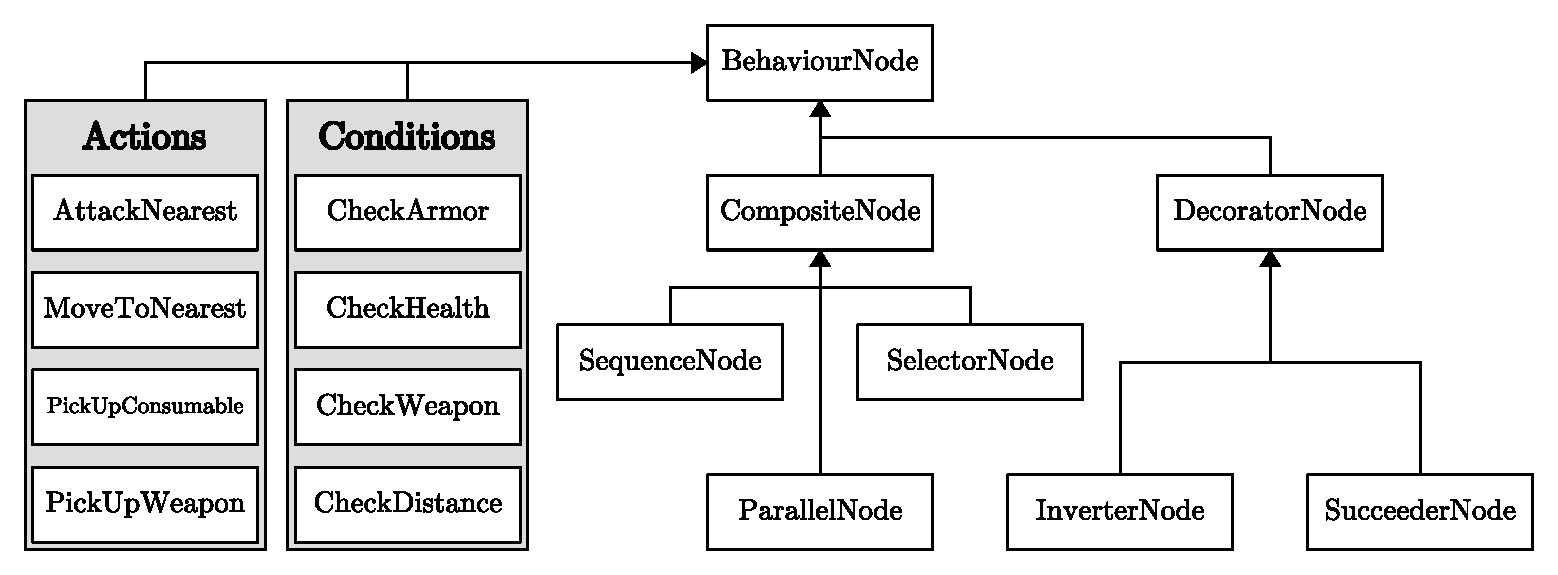
\includegraphics[width=\textwidth]{share/behaviour_tree_uml.eps}
            \caption{Class hierarchy overview of our behaviour tree implementation in Java. Based on BT-SK~\cite{champandard2014behaviour}.}
            \label{fig:behaviour_tree_hierarchy}
            \twocolumn
        \end{figure}

        \subsection{Behaviour Trees} \label{sec:behaviour_trees_implementation}

        Inside of \texttt{se.sciion.quake2d.ai.behaviour} you'll find the implementation of our BTs. They are specified using inheritance, as shown in \cref{fig:behaviour_tree_hierarchy}. In our variant, only the leaves above are non-abstract.

        All are derived from the \texttt{BehaviourNode}, which provides the \emph{State}, and methods for updating states, by evaluating it and its children (if it has any). This is done with the \texttt{tick} function, which is called for each agent's behaviour tree and once for each frame.

        \vspace{-0.4em}

        \begin{algorithm}
            \caption{Pseudo-Code for the BT's Tick Step}
            \label{alg:behaviour_tree_update}
            \begin{algorithmic}
                \REQUIRE{some initial \(State\) to the behaviour tree}
                \IF{\(State \neq Running\)}
                    \STATE \(doBehaviourEnter()\)
                \ENDIF
                \STATE \(State \leftarrow doBehaviourUpdate()\)
                \IF{\(State \neq Running\)}
                    \STATE \(doBehaviourExit()\)
                \ENDIF
            \end{algorithmic}
        \end{algorithm}

        \vspace{-0.6em}

        In each of these entities' behaviour tree, built from the bottom-up and linked, there is one \texttt{root} node. Only this node needs to be evaluated, since the root will recursively evaluate its children when requested.

        The standard non-leaf nodes are implemented in a straight-forward way following \cref{sec:behaviour_trees}. Instead, we concentrate on explaining \emph{actions} and \emph{conditions} we have implemented, and how these communicate with the other systems to be able to query the world.

        We've adopted a fairly simple solution, where the leaf-node is given a reference to systems that it wants to communicate with, and a entity owner too.

        \hfill\vspace{19.4em}

        For example, if a BT wants a \emph{AttackNearest} node beneath a \emph{Succeeder}, we'd first have to hand over a reference to the \emph{path finder} and a \emph{target tag} to the constructed node: \emph{AttackNearest(path-finder, tag)}. Only after that we: \emph{SucceederNode(attack-nearest)}, which we can use to build a next layer above itself.

        Below is a list of all actions and conditions we've implemented in our game, along with a description:

        \begin{itemize}
            \item{\textbf{AttackNearest(\emph{tag}):} finds the closest entity with \emph{tag} and \emph{path find} to it. Shoot with weapon. \emph{Success} if we were able to fire, \emph{false} otherwise.}
            \item{\textbf{MoveToNearest(\emph{tag}):} finds the close entity with \emph{tag} and \emph{path find} to it. Stops when close. \emph{Success} when we're close, \emph{fails} if no valid path.}
            \item{\textbf{PickUpConsumable(\emph{type}):} finds the closest consumable of \emph{type} (\emph{health}, \emph{armor} and \emph{boost}), \emph{path find} to it and \emph{pick it up}. \emph{Fails} if it can't...}
            \item{\textbf{PickUpWeapon(\emph{type}):} finds a close weapon of \emph{type} (\emph{shotgun}, \emph{rifle} \& \emph{sniper}). \emph{Path find} to it \& try to \emph{pick it up}. \emph{Succeeds} when picked up.}
        \end{itemize}

        \begin{itemize}
            \item{\textbf{CheckArmor(\emph{ratio}):} checks entity owner's \emph{armor}, gives \emph{Success} if above \emph{ratio}, \emph{fail} if below.}
            \item{\textbf{CheckHealth(\emph{ratio}):} checks entity owner's \emph{health}, gives \emph{Success} if above \emph{ratio}, \emph{fail} if below.}
            \item{\textbf{CheckWeapon(\emph{type}):} checks entity owner's \emph{inventory} for weapon \emph{type}. \emph{Success} if we got it.}
            \item{\textbf{CheckDistance(\emph{tag, r})} checks if entity with \emph{tag} is above \emph{r} units away. \emph{Succeeds} query if so.}
        \end{itemize}

        \clearpage

        \subsection{Genetic Programming} \label{sec:genetic_programming_implementation}

        All BTs generated for the \textit{genetic programming} optimization has to be generated during \textit{runtime}. This is done by creating an set \(\mathcal{P}\) with a \textit{prototype object} (following the \textit{prototype pattern}~\cite{nystrom2014game}) of each \textit{behaviour node} \(p\).

        \textbf{Behaviour tree generation}: Each \textit{behaviour node prototype} contains a function which causes the node to randomize it self \(\rho(p)\). For leaf nodes this means tweaking parameters such as \textit{thresholds} and \textit{entity tags}
        \begin{equation*}
            \rho(p) \rightarrow \hat{p}
        \end{equation*}
        where \(\hat{p}\) is a new instance of the same behaviour type as \(p\).

        Composite nodes, it involves changing the children \(\{n_0,n_1,...,n_m\} \in p\) on the form:
        \begin{equation*}
            \rho(p) \rightarrow \forall_{n \in p}{\rho(n)}
        \end{equation*}
        which given that \(n_k\) can be a composite as well, allows for creation of all possible trees which the prototypes in \(\mathcal{P}\) can define. This can be seen as each tree representing a sentence in the regular grammar of the alphabet \(\mathcal{P}\).

        \textbf{Mutation of nodes}: As with the \textit{randomization}, the mutation of BTs are done in a recursive manner where each node mutate it self, and in the case of composite nodes, also its children. The mutation function \(\mu(p)\) is defined as \(\mu(p) \rightarrow \hat{p}\) for leaf nodes and 
        \begin{align*}
            \mu(p) &\rightarrow \forall_{n \in p}{\mu(n)} \\
            \mu(p) &\rightarrow \{p_0,p_1,...,p_k,n_0,m_1,...,n_m\}, p_n \in \mathcal{P}, k \in \mathbf{R} \\
        \end{align*}
        where the first definition mutates the existing children and the second adds \(k\) new nodes \(\{p_0,p_1,...,p_k\}\) to the child set.

    \clearpage

    \section{Results and Screenshots} \label{sec:results_and_screenshots}

        Below are a couple of in-game screenshots from \emph{Quake 2D}, our testbed for \emph{behaviour tree evolution}. Here we've chosen to show two bots playing against each other in the arena, each of them loaded with a basic hand-made behaviour tree shown in \cref{fig:hand_crafted_behaviour_tree}.

        \begin{figure}[H]
            \centering
            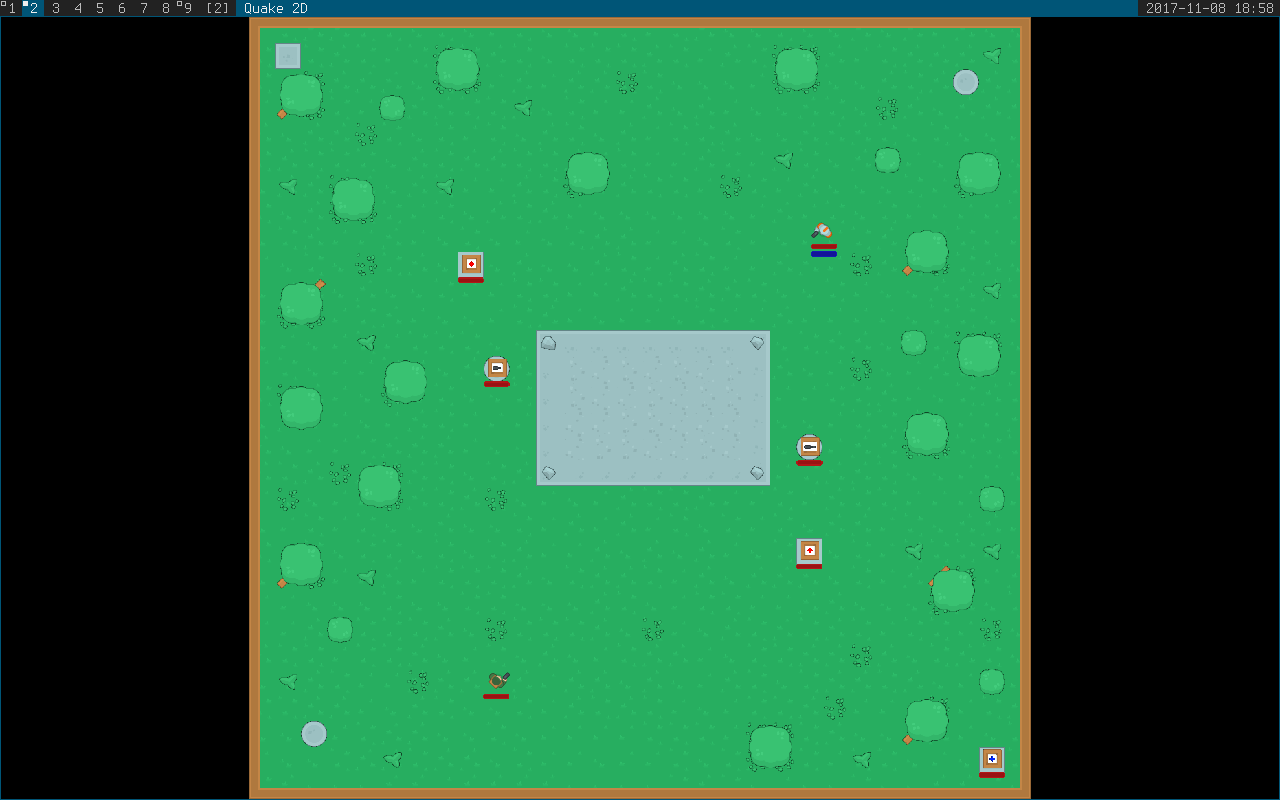
\includegraphics[width=\linewidth]{share/screenshot.png}
            \caption{Screenshot of a Bot vs Bot in Quake 2-D}
            \label{fig:behaviour_tree_screenshot}
        \end{figure}

        \begin{figure}[H]
            \centering
            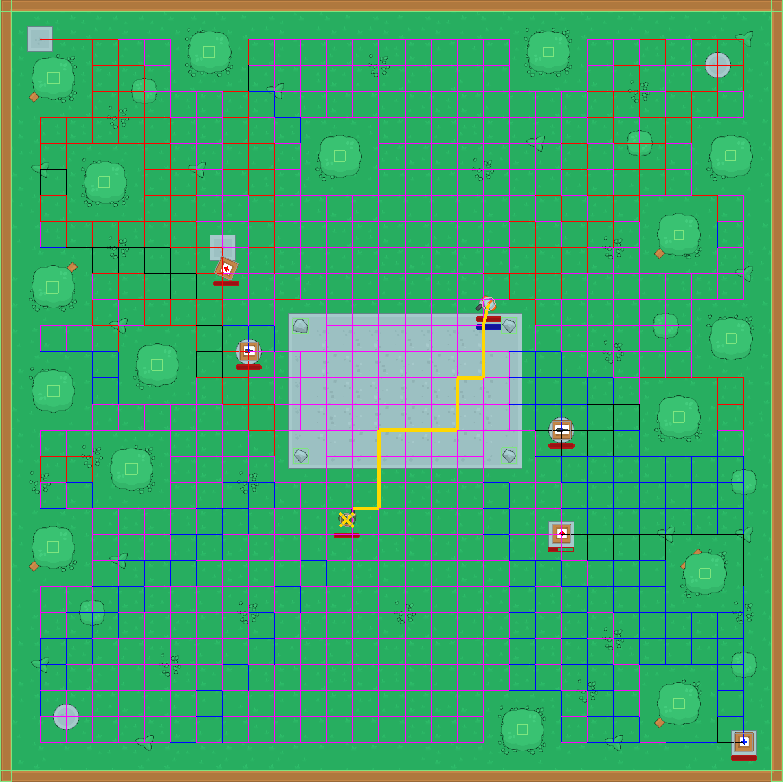
\includegraphics[width=\linewidth]{share/path_finding_screenshot.png}
            \caption{Screenshot of Path Finding in Quake 2-D}
            \label{fig:path_finding_screenshot}
        \end{figure}

        \begin{figure}[H]
            \centering
            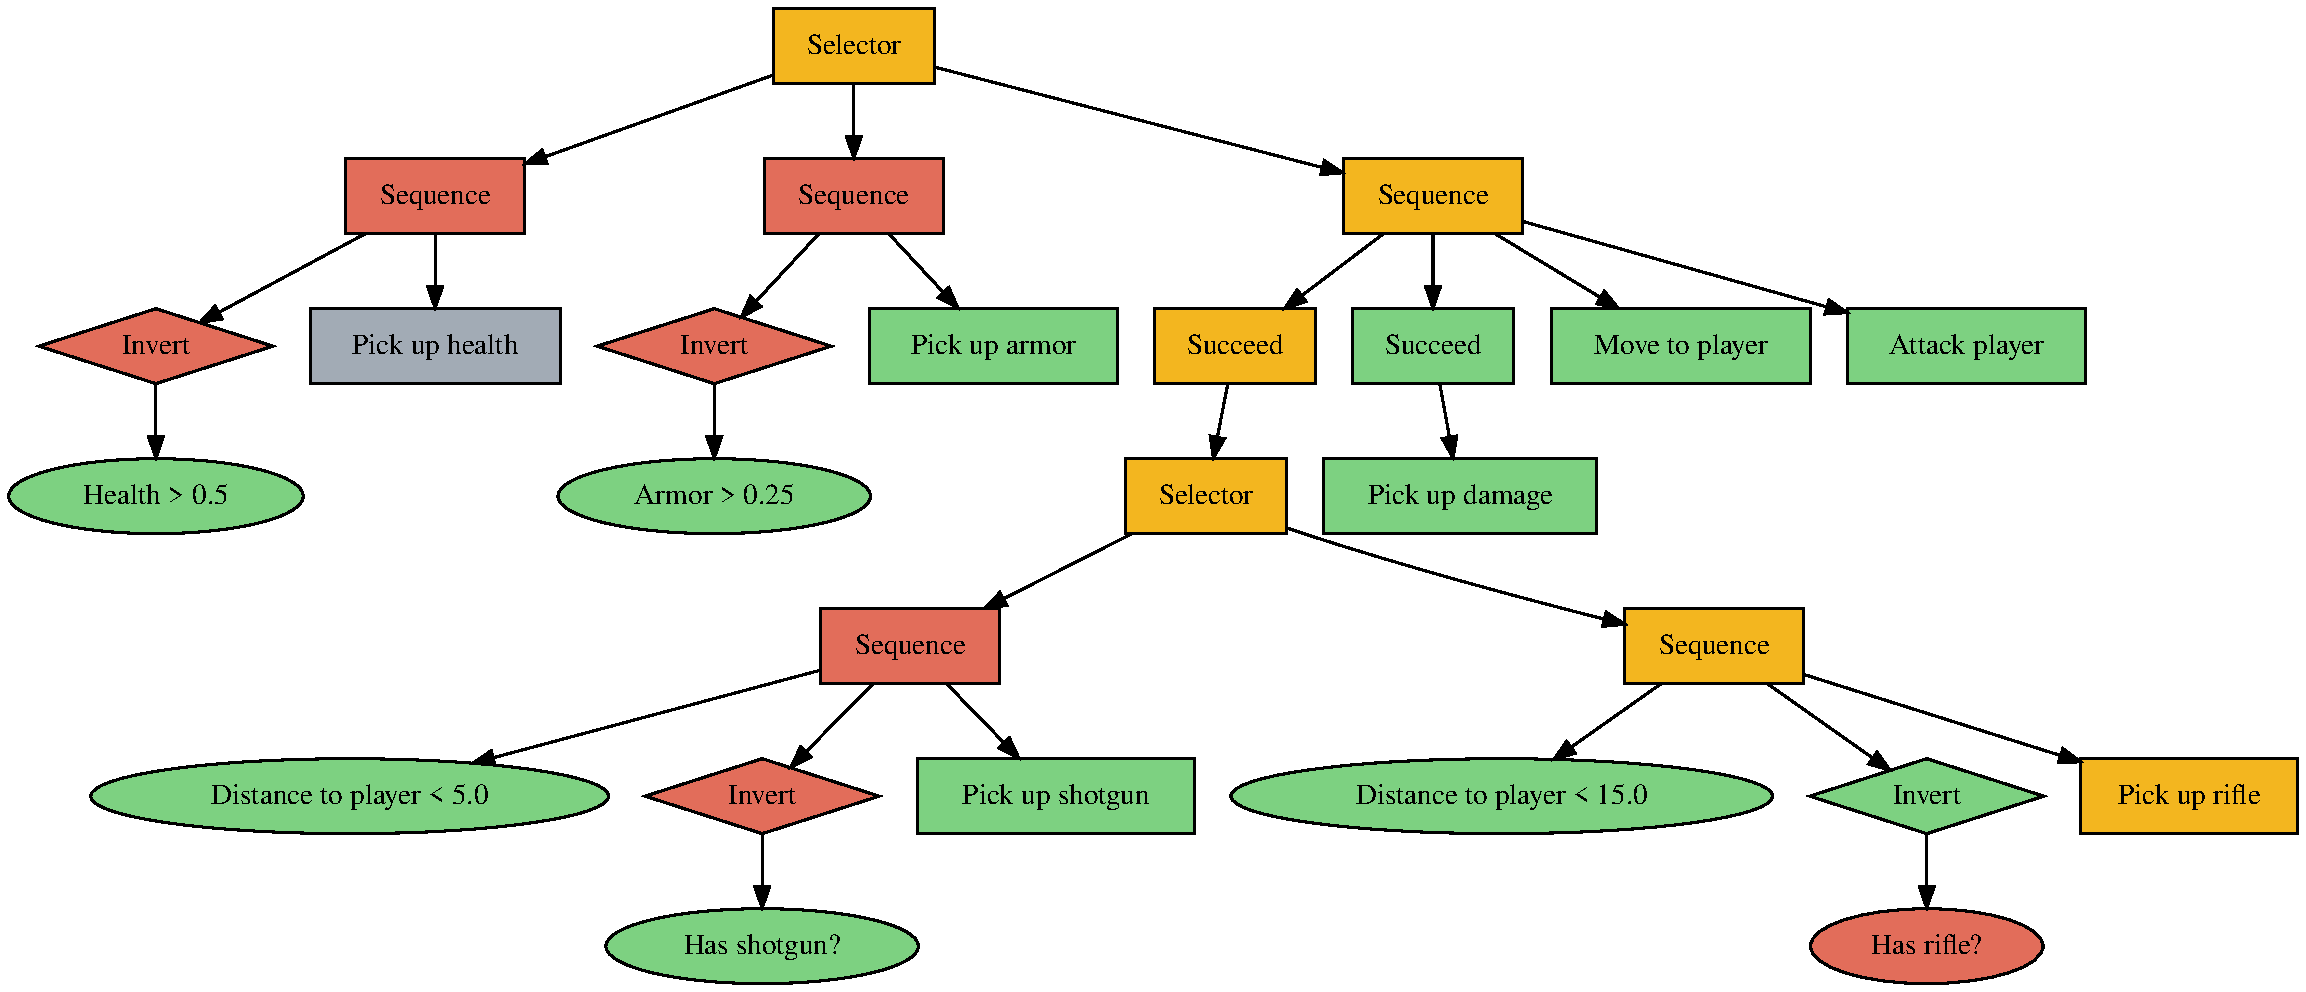
\includegraphics[width=\linewidth]{share/hand_crafted_behaviour_tree.pdf}
            \caption{A Hand-Crafted BT (Larger in Appendix)}
            \label{fig:hand_crafted_behaviour_tree}
        \end{figure}

        \subsection{Generated Behaviours} \label{sec:generated_behaviours}



        \subsection{Behaviour Fitness} \label{sec:behaviour_fitness}



        \subsection{Survival Rate} \label{sec:survival_rate}



    \section{Discussion and Outlook} \label{sec:discussion_and_outlook}

    \onecolumn
    \clearpage

    \appendix
    \thispagestyle{empty}

    \begin{figure}[H]
        \centering
        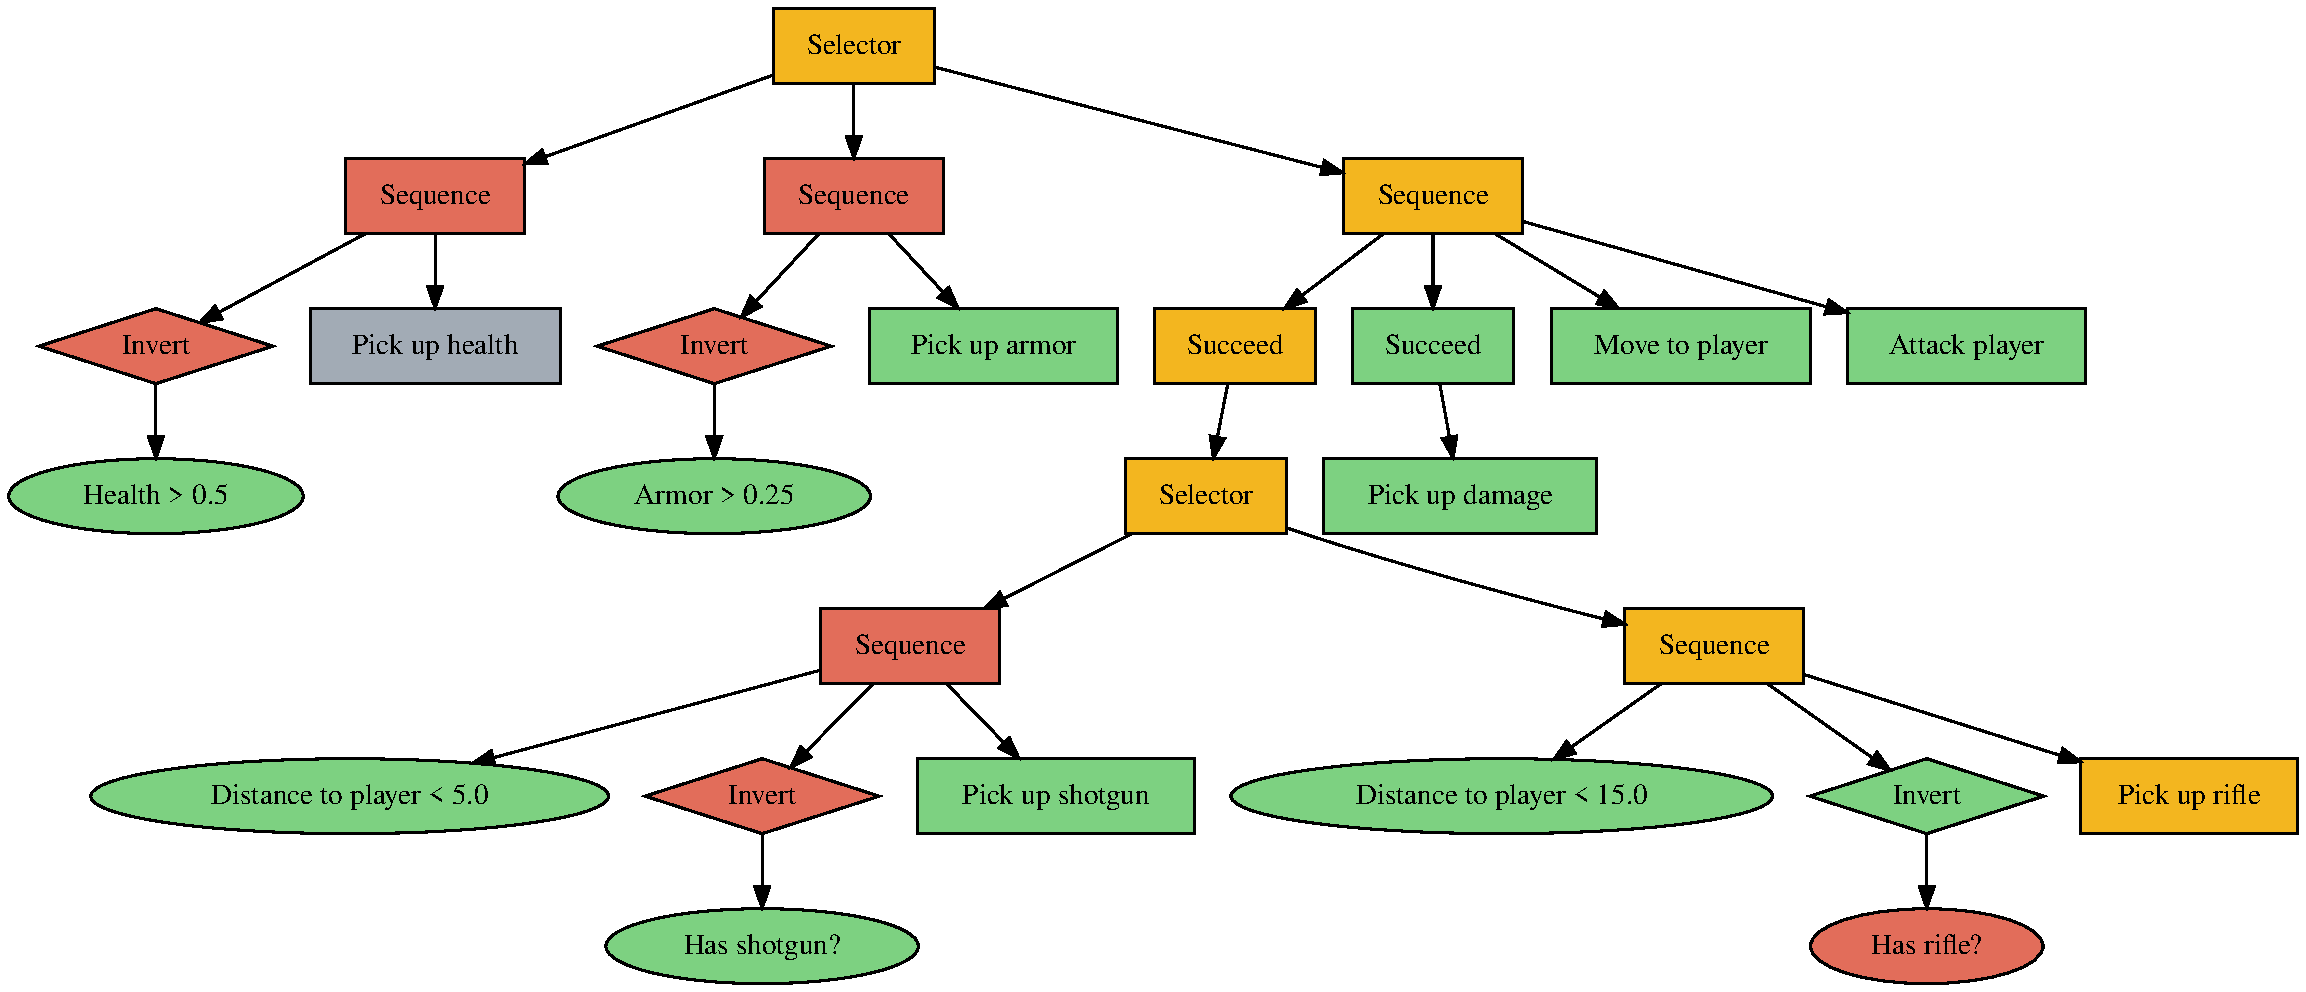
\includegraphics[angle=90,height=0.98\textheight]{share/hand_crafted_behaviour_tree.pdf}
    \end{figure}

\end{document}
